\documentclass[11pt, a4paper, titlepage]{article}
\setlength{\parindent}{0pt} % quitamos indentacion automática en parrafos

% \addtolength{\textwidth}{+100cm}

\usepackage[utf8]{inputenc}
\usepackage[T1]{fontenc}
\usepackage[spanish]{babel}
% \usepackage{lmodern}
\usepackage{blindtext}
\usepackage{vmargin}
\usepackage[hidelinks]{hyperref}
\usepackage{url}
\usepackage{lipsum}
\usepackage{adforn} % símbolo lista
\usepackage{graphicx}


 
\usepackage{color}
\usepackage{csquotes}   
\usepackage[style=numeric-comp, sorting=none, block=par]{biblatex} 
\addbibresource{references.bib}
\DeclareFieldFormat{title}{\bfseries\emph{#1}}
\definecolor{softblack}{RGB}{74, 71, 71} 
\DeclareFieldFormat{howpublished}{\textcolor{softblack}{\mdseries{#1}}}
\DeclareFieldFormat{labelnumberwidth}{\mkbibbold{#1\adddot}}
\setlength\bibitemsep{2.5\itemsep}
\renewcommand*{\newunitpunct}{\addspace}
\renewcommand*{\finentrypunct}{\addspace}
% \renewcommand\mkbibnamefamily[1]{\textbf{#1}}

% \usepackage{xurl} % tiene que estar despues de biblatex

\usepackage{tocloft}
% \setlength{\cftbeforesecskip}{6pt}
\setlength{\cftbeforesubsecskip}{6pt}
\setlength{\cftbeforesubsubsecskip}{3pt}


\usepackage{titlesec}
\definecolor{gray75}{gray}{0.75}
\newcommand{\hsp}{\hspace{20pt}}
\titleformat{\section}[hang]{\LARGE\bfseries}{\thesection\hsp\textcolor{gray75}{|}\hsp}{0pt}{\LARGE\bfseries}
\titlespacing{\section}{0pt}{0pt}{15pt}
\titleformat{\subsection}[hang]{\Large\bfseries}{\thesubsection\hsp}{0pt}{\Large\bfseries}
\titlespacing{\subsection}{0pt}{35pt}{15pt}
\titleformat{\subsubsection}[hang]{\large\bfseries}{\thesubsubsection\hspace{10pt}}{0pt}{\large\bfseries} 
\titlespacing{\subsubsection}{0pt}{20pt}{0pt}


\newenvironment{myitemize}
{ \begin{itemize}
    \setlength{\itemsep}{0pt}
    \setlength{\parskip}{2pt}    }
{ \end{itemize}                  } 
    
\newcommand{\minus}{\scalebox{0.75}[1.0]{$-$}}
    
\newenvironment{changemargin}[2]{%
\begin{list}{}{%
\setlength{\topsep}{0pt}%
\setlength{\leftmargin}{#1}%
\setlength{\rightmargin}{#2}%
\setlength{\listparindent}{\parindent}%
\setlength{\itemindent}{\parindent}%
\setlength{\parsep}{\parskip}%
}%
\item[]}{\end{list}}


\usepackage[dvipsnames]{xcolor}

\renewcommand*{\ttdefault}{\familydefault}

\usepackage{fancyvrb}

% redefine \VerbatimInput
\RecustomVerbatimCommand{\VerbatimInput}{VerbatimInput}%
{fontfamily=cmr, %esto ya no hace falta al poner ttdefault
 codes={\catcode`$=3},
 commandchars=\#\[\] % escape character and argument delimiters for
                       % commands within the verbatim
}


% \usepackage{geometry}
%  \geometry{
%  a4paper,
%  total={210mm,297mm},
%  left=60mm,
%  right=20mm,
%  top=40mm,
%  bottom=20mm,
%  }
 
% \usepackage{fancyhdr}

% \pagestyle{fancy}
% \fancyhead[LO,LE]{Curso 2020/2021}
% \fancyhead[CO,CE]{Grado en Ingeniería Informática}
% \fancyfoot[CO,CE]{\thepage}

% \renewcommand{\headrulewidth}{0.4pt} % grosor de la línea de la cabecera
% \renewcommand{\footrulewidth}{0.4pt} % grosor de la línea del pie
% \usepackage{pdfpages} % to include external pdf's

% \setpapersize{A4}
% \setmargins{2.5cm}       % margen izquierdo
% {1cm}                        % margen superior
% {16.5cm}                      % anchura del texto
% {23.42cm}                    % altura del texto
% {10pt}                           % altura de los encabezados
% {2cm}                           % espacio entre el texto y los encabezados
% {0pt}                             % altura del pie de página
% {2cm}                           % espacio entre el texto y el pie de página

% \usepackage{geometry}
%  \geometry{
%  a4paper,
%  total={170mm,257mm},
%  left=20mm,
%  top=20mm,
%  }

% \title{Ejercicio Individual II}
% \author{Daniel Tomás Sánchez\\ asdas\\ dfsf}
% \date{Diciembre 2020}

\begin{document}
% Cuerpo del documento
\begin{titlepage}
    \begin{center}
        \hrulefill

        \vspace{0.5cm}
        {\bfseries\Huge Procesadores de Lenguajes \par}
        \vspace{3cm}

        {\scshape \LARGE \textbf{Memoria Final}}

        \hrulefill

        \vspace{2.0cm}
    \end{center}

    \centering

    % {\scshape\Huge\textbf{}\par}
    % \vspace{1cm}
    % {\scshape\Huge\textbf{Ejercicio Individual II}\par}
    % \vspace{3cm}

    \Large{Grupo 55}\\
    \vspace{0.3cm}

    {\large Daniel Tomás Sánchez\\ Aarón Cabero Blanco\\ Alejandro Cuadrón \par}

    \vspace{2cm}
    {\Large Curso 2020/2021 \par}
\end{titlepage}

%\maketitle

% \clearpage
\tableofcontents
\clearpage


\section{Introducción}
El trabajo completo, tanto el léxico, como el sintáctico y el semático, ha sido realizado con la herramienta o librería externa "SLY" \cite{SLY}.\\

Opciones de grupo:
\begin{myitemize}
    \renewcommand{\labelitemi}{$\circ$}
    \item Sentencias: Sentencia repetitiva (\textbf{for})
    \item   Operadores especiales: Post-auto-decremento (\textbf{\minus \minus \hspace{0.1cm} como sufijo})
    \item     Técnicas de Análisis Sintáctico: \textbf{Ascendente}
    \item     Comentarios: Comentario de bloque (\textbf{/* */})
    \item Cadenas: Con comillas dobles (\textbf{" \phantom{} "})
\end{myitemize}
\clearpage

\section{Diseño Analizador Léxico}

% % LO SUYO hubiese sido hacerlo asi
% \newcommand{\fila}[2]{$\bullet$ & #1 & <#2>\\}
% \begin{tabular}{cll}
% \fila{Identificador}{ID, punteroTS}
% \fila{Palabra reservada Number}{<NUMBER, ->}
% \end{tabular}

\begin{changemargin}{0cm}{+4cm}
    \subsection{Tokens}
    \begin{flushleft}
        \begin{myitemize}
            \item Identificador \hfill<ID, punteroTS>
            \item Constante entera \hfill<CTEENTERA, valor>
            \item Cadena de caracteres \hfill<CADENA, lexema>
            \item false \hfill<CTELOGICA, 0>
            \item true \hfill<CTELOGICA, 1>
            \item Palabra reservada Number\hfill<NUMBER, ->
            \item Palabra reservada String\hfill<STRING, ->
            \item Palabra reservada Boolean\hfill<BOOLEAN, ->
            \item Palabra reservada Let\hfill<LET, ->
            \item Palabra reservada Alert\hfill<ALERT, ->
            \item Palabra reservada Input\hfill<INPUT, ->
            \item Palabra reservada Function\hfill<FUNCTION, ->
            \item Palabra reservada Return \hfill<RETURN, ->
            \item Palabra reservada If \hfill<IF, ->
            \item Palabra reservada For\hfill<FOR, ->
            \item \minus \minus \hfill<OPESP, ->
            \item \minus  \hfill<OPARIT, ->
            \item =\hfill <OPASIG, ->
            \item == \hfill<OPREL, ->
            \item \&\& \hfill<OPLOG, ->
            \item ( \hfill<ABPAREN, ->
                  \item ) \hfill<CEAPAREN,>
            \item \{ \hfill<ABLLAVE, ->
            \item \} \hfill<CELLAVE, ->
            \item , \hfill<COMA, ->
            \item ; \hfill<PUNTOYCOMA, ->
        \end{myitemize}
    \end{flushleft}
\end{changemargin}
\clearpage

\subsection{Gramática Regular}
\noindent
Axioma = A\\
A $\rightarrow$ del A $|$ d D $|$ " \hspace{1mm} S $|$ / C $|$ l I $|$ \minus  M $|$ = E $|$ \& N $|$ ( $|$ ) $|$ \{ $|$ \} $|$ ; $|$ , \\
D $\rightarrow$ d D $|$ $\lambda$\\
S $\rightarrow$ " \hspace{1mm} $|$ c S\\
C $\rightarrow$ * C'\\
C' $\rightarrow$ * C'' $|$ c C'\\
C'' $\rightarrow$ / A $|$ c C'\\
I $\rightarrow$ d I $|$ l I $|$ \_ I $|$ $\lambda$\\
M $\rightarrow$ \minus \hspace{1.5mm}$|$ $\lambda$\\
E $\rightarrow$ = $|$ $\lambda$\\
N $\rightarrow$ \&\\
\\
Siendo $d$ un dígito, $l$ una letra, $c$ cualquier otro carácter y $del$ un delimitador.

\subsection{Autómata Finito Determinista}
\begin{center}
    % 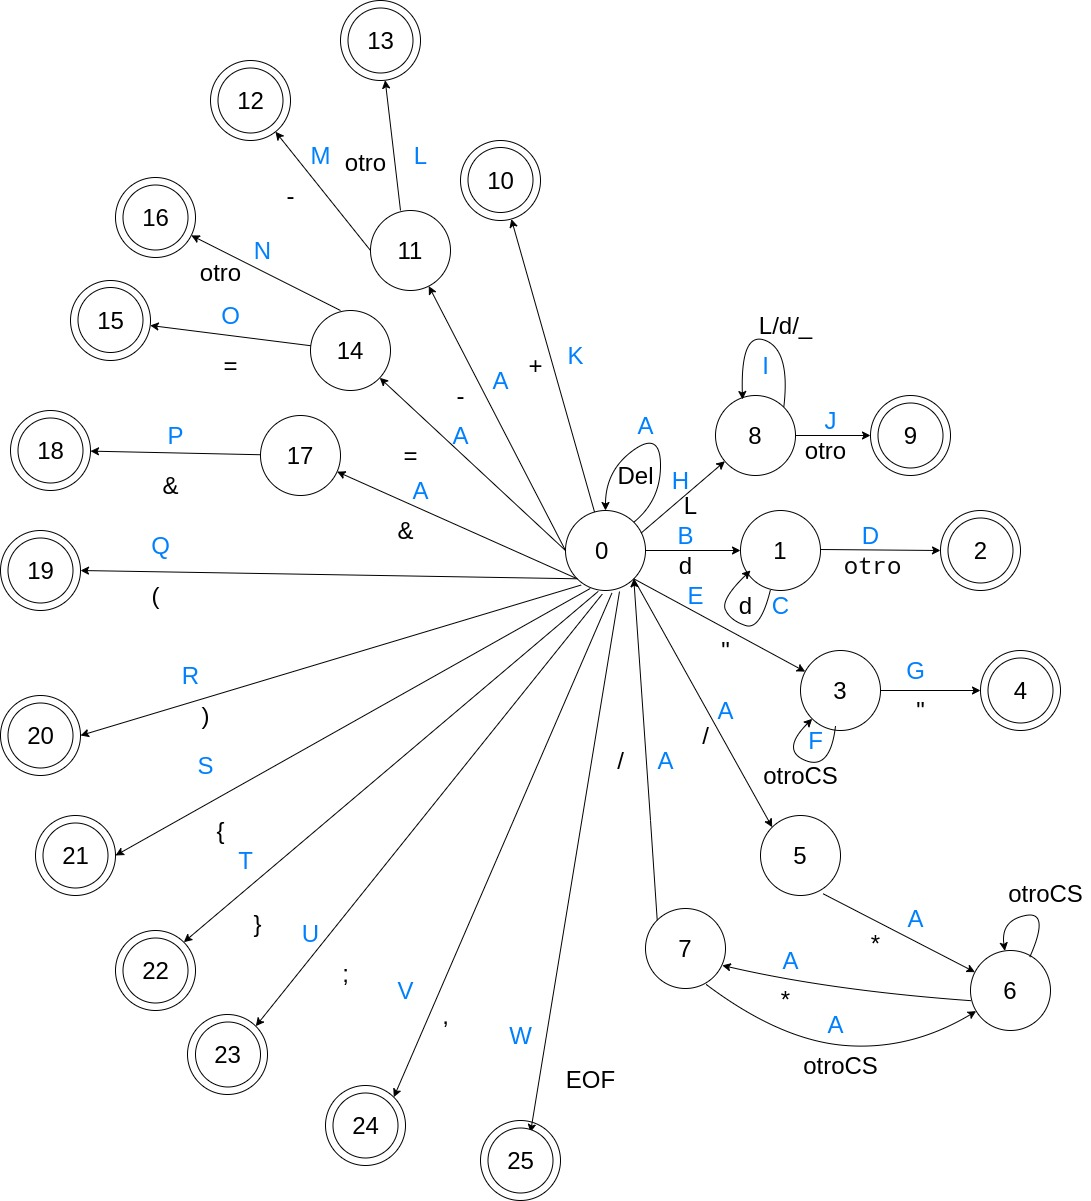
\includegraphics[scale=0.33]{automata.jpg}
\end{center}
\clearpage

\subsection{Acciones Semánticas}
\begin{flushleft}
    A: leer\\
    B: number = int(d), leer\\
    C: number = number * 10 + int(d), leer\\
    D: if number >\hspace{1mm} 32767\\
    \qquad pError("Número fuera de rango")\\
    \quad else \\
    \qquad genToken(CTEENTERA, number);\\
    E: string = \verb|""|, contador = 0, leer\\ 
    F: string = string + otroCS, contador++, leer\\
    G: if contador >\hspace{1mm} 64\\
    \qquad pError(\verb|"Cadena| demasiado larga")\\
    \quad else\\
    \qquad genToken(CADENA, string)\\
    \quad leer\\
    H: string = l, leer\\
    I: string = string + l/D/\_ , leer\\
    J: if palabrasReservadas.contains(string)\\
    \qquad if string == "number"\\
    \qquad \quad      genToken(NUMBER, -)\\
    \qquad elif string == "string"\\
    \qquad \quad     genToken(STRING,-)\\
    \qquad  elif string == "boolean"\\
    \qquad \quad      genToken(BOOLEAN, -)\\
    \qquad    elif string == "let"\\
    \qquad \quad      genToken(LET, -)\\
    \qquad    elif string == "\phantom{}alert"\\
    \qquad \quad      genToken(ALERT, -)\\
    \qquad    elif string == "\phantom{}input"\\
    \qquad \quad      genToken(INPUT, -)\\
    \qquad    elif string == "\phantom{}return"\\
    \qquad \quad       genToken(RETURN, -)\\
    \qquad     elif string == "\phantom{}if"\\
    \qquad \quad       genToken(IF, -)\\
    \qquad     else\\
    \qquad \quad      genToken(FOR, -)\\
    \clearpage
    \quad       else \hspace{5mm} // palabrasReservadas.contains(string) = False\\
    \qquad          puntero = TS.get(string)\\
    \qquad          if zona\_decl == True\\
    \qquad \quad        if puntero != None\\
    \qquad \quad \quad      pError("\phantom{}Identificador ya declarado")\\
    \qquad \quad        else\\
    \qquad \quad \quad      TS.update({string})\\
    \qquad \quad \quad      puntero = TS.get(string)\\
    \qquad \quad \quad      genToken(ID, puntero)\\
    \qquad          else\\
    \qquad \quad        if puntero == None\\
    \qquad \quad \quad      TS.update({string})\\
    \qquad \quad \quad      puntero = TS.get(string)\\
    \qquad \quad \quad      genToken(ID, puntero)\\
    \qquad \quad        else\\
    \qquad \quad \quad      genToken(ID, puntero)\\
    \vspace{\baselineskip}
    L: genToken(OPARIT, -)\\
    M: genToken(OPESP, -), leer\\
    N: genToken(OPASIG, -)\\
    O: genTokeN(OPREL, -), leer\\
    P: genToken(OPLOG, -), leer\\
    Q: genToken(ABPAREN, -), leer\\
    R: genToken(CEPAREN, -), leer\\
    S: genToken(ABLLAVE, -), leer\\
    T: genToken(CELLAVE, -), leer\\
    U: genToken(COMA, -), leer\\
    V: genToken(PUNTOYCOMA, -), leer\\
    W: genToken(EOF, -), leer\\
\end{flushleft}

\subsection{Errores}
Error léxico (siempre se lanza cuando el analizador léxico encuentra un error).
\begin{enumerate}
    \item Cadena con longitud mayor de 64 caracteres.
    \item Número fuera de rango (mayor de 32767).
    \item Identificador ya declarado.
    \item Carácter ilegal.
\end{enumerate}
Todo error va acompañado de la $linea$ y $columna$ en el que se ha encontrado dicho error.
\clearpage

\section{Diseño Analizador Sintáctico}

\subsection{Gramática}
Axioma = B\\
No Terminales = \{ A B C D E F G H I J K L M N O P Q R S T U V W F1 F2 F3 \}\\
Terminales = \{ \&\& == \minus \hspace{0.1cm} \minus\minus \hspace{0.1cm} (\hspace{0.1cm}  ) =\hspace{0.1cm}  ,\hspace{0.1cm}  ; { } id %
ent cad log let alert input return for if number\\
\hspace*{2.65cm}boolean string function \}\\\\
Producciones = \{\\
\setlength{\tabcolsep}{1.5cm}
\begin{tabular}{ l l }
    B $\rightarrow$ D                       & O $\rightarrow$ $\lambda$                      \\
    D $\rightarrow$ F D                     & C $\rightarrow$ G C                            \\
    D $\rightarrow$ G D                     & C $\rightarrow$ $\lambda$                      \\
    D $\rightarrow$ $\lambda$               & F $\rightarrow$ F1 F2 F3                       \\
    G $\rightarrow$ if ( E ) S              & F1 $\rightarrow$ function P Q id               \\
    G $\rightarrow$ S                       & P $\rightarrow$ $\lambda$                      \\
    S $\rightarrow$ H ;                     & Q $\rightarrow$ T                              \\
    H $\rightarrow$ id ( I )                & Q $\rightarrow$ $\lambda$                      \\
    I $\rightarrow$ E J                     & F2 $\rightarrow$ ( A )                         \\
    I $\rightarrow$ $\lambda$               & A $\rightarrow$ T id AA                        \\
    J $\rightarrow$ , E J                   & A $\rightarrow$ $\lambda$                      \\
    J $\rightarrow$ $\lambda$               & AA $\rightarrow$ , T id AA                     \\
    S $\rightarrow$ K ;                     & AA $\rightarrow$ $\lambda$                     \\
    K $\rightarrow$ id = E                  & F3 $\rightarrow$ { C }                         \\
    S $\rightarrow$ alert ( E ) ;           & E $\rightarrow$ E \&\& R                       \\
    S $\rightarrow$ input ( id ) ;          & E $\rightarrow$ R                              \\
    S $\rightarrow$ return L ;              & R $\rightarrow$ R == U                         \\
    L $\rightarrow$ E                       & R $\rightarrow$ U                              \\
    L $\rightarrow$ $\lambda$               & U $\rightarrow$ U \minus\hspace{0.1cm} V       \\
    G $\rightarrow$ let M T id ;            & U $\rightarrow$ V                              \\
    M $\rightarrow$ $\lambda$               & V $\rightarrow$ \minus\minus \hspace{0.1cm} id \\
    T $\rightarrow$ number                  & V $\rightarrow$ id                             \\
    T $\rightarrow$ boolean                 & V $\rightarrow$ ( E )                          \\
    T $\rightarrow$ string                  & V $\rightarrow$ H                              \\
    G $\rightarrow$ for ( N ; E ; O ) { C } & V $\rightarrow$ ent                            \\
    N $\rightarrow$ K                       & V $\rightarrow$ cad                            \\
    N $\rightarrow$ $\lambda$               & V $\rightarrow$ log                            \\
    O $\rightarrow$ K                                                                        \\
    O $\rightarrow$ \minus\minus \hspace{0.1cm} id
\end{tabular}
\\\}
\clearpage

\subsection{Tabla LR(1) }
\begin{changemargin}{-2.5cm}{+2.5cm}
    \begin{center}
        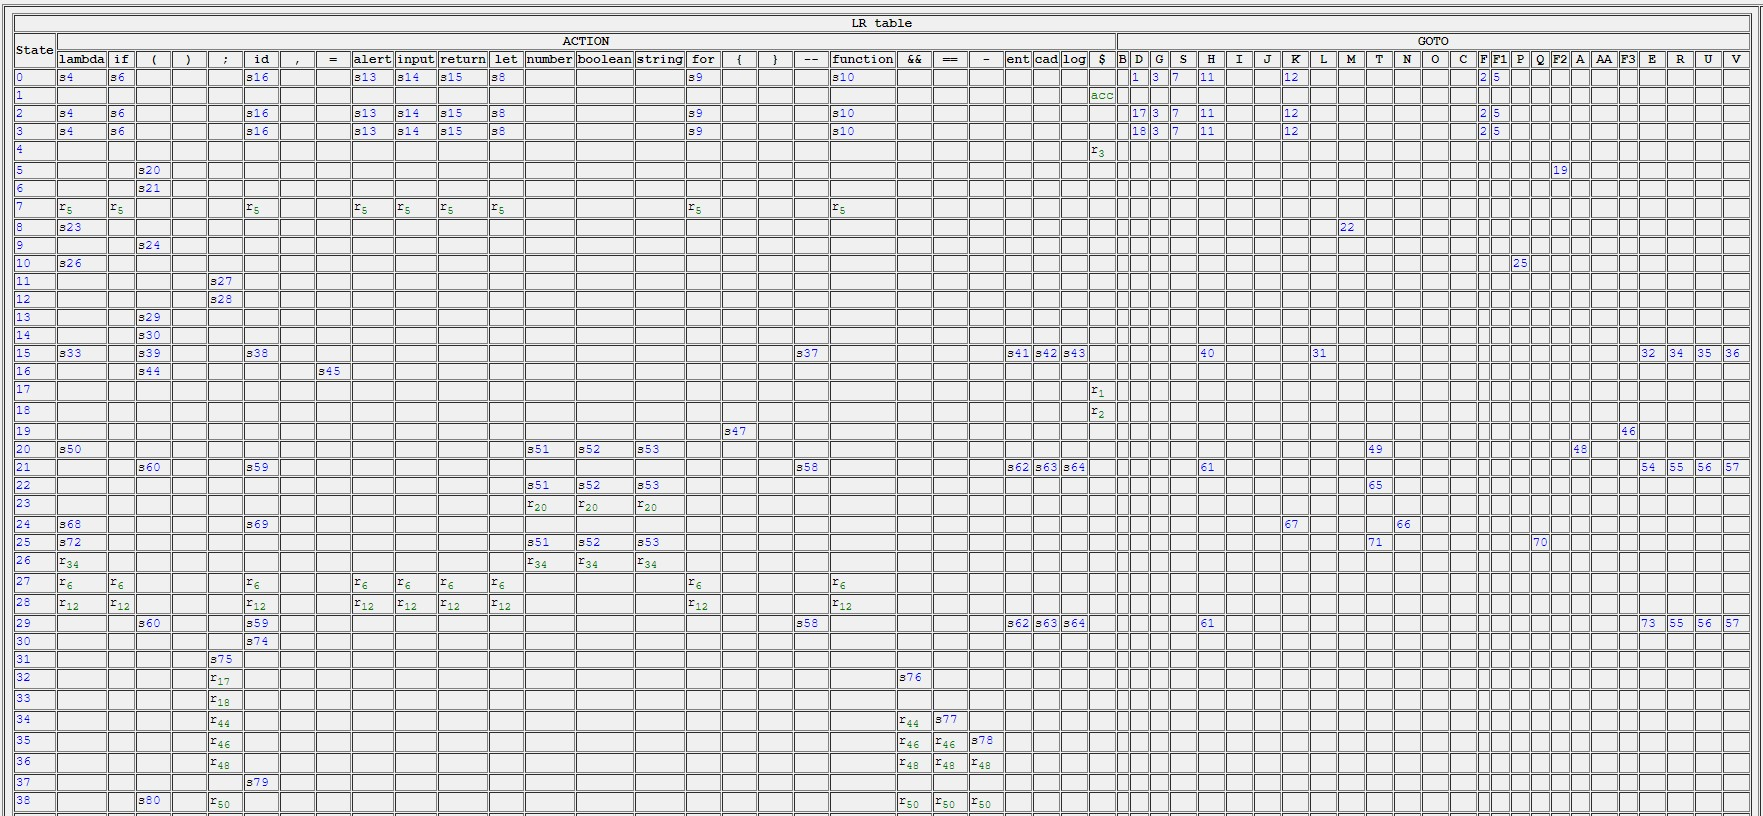
\includegraphics[width=1.27\textwidth]{Tabla1.jpg}
        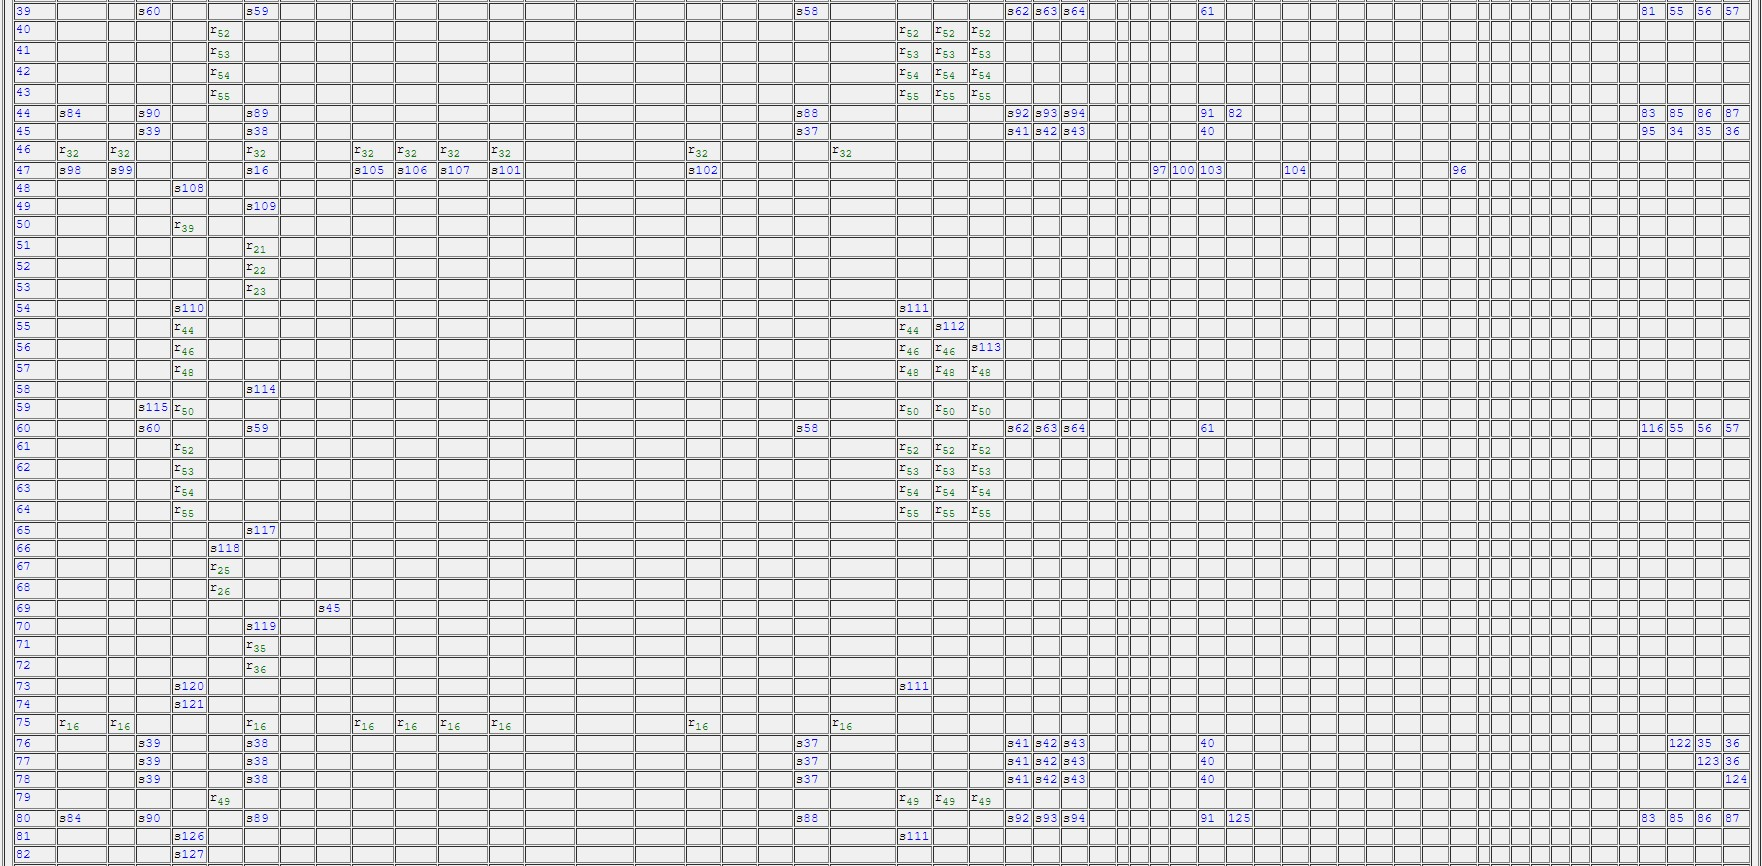
\includegraphics[width=1.27\textwidth]{Tabla2.jpg}
        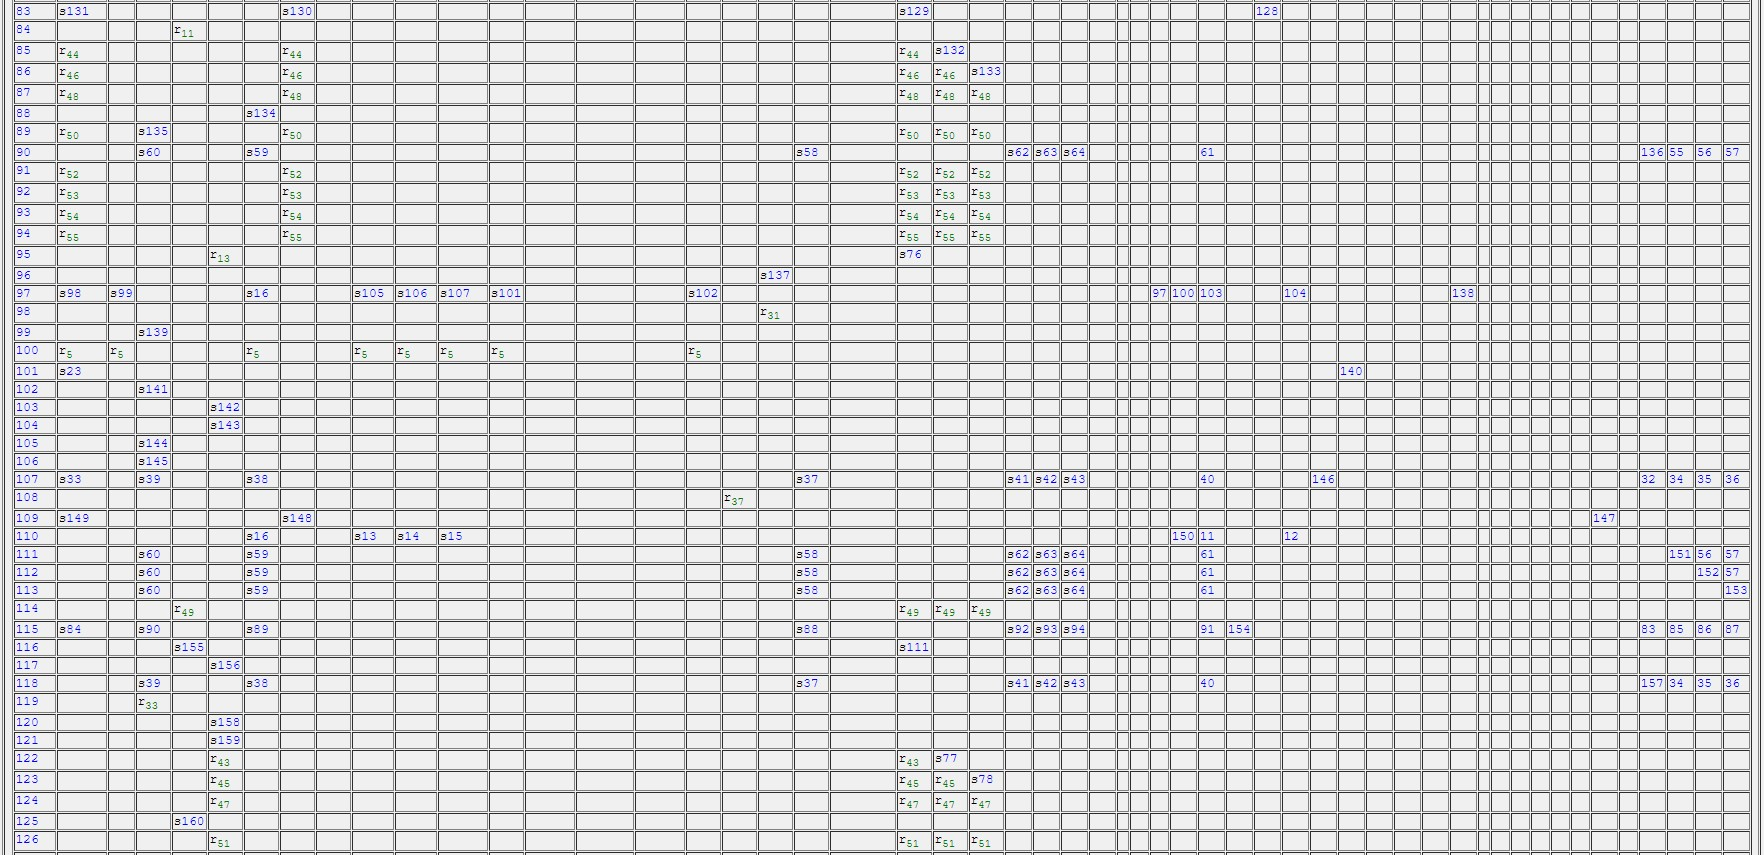
\includegraphics[width=1.27\textwidth]{Tabla3.jpg}
        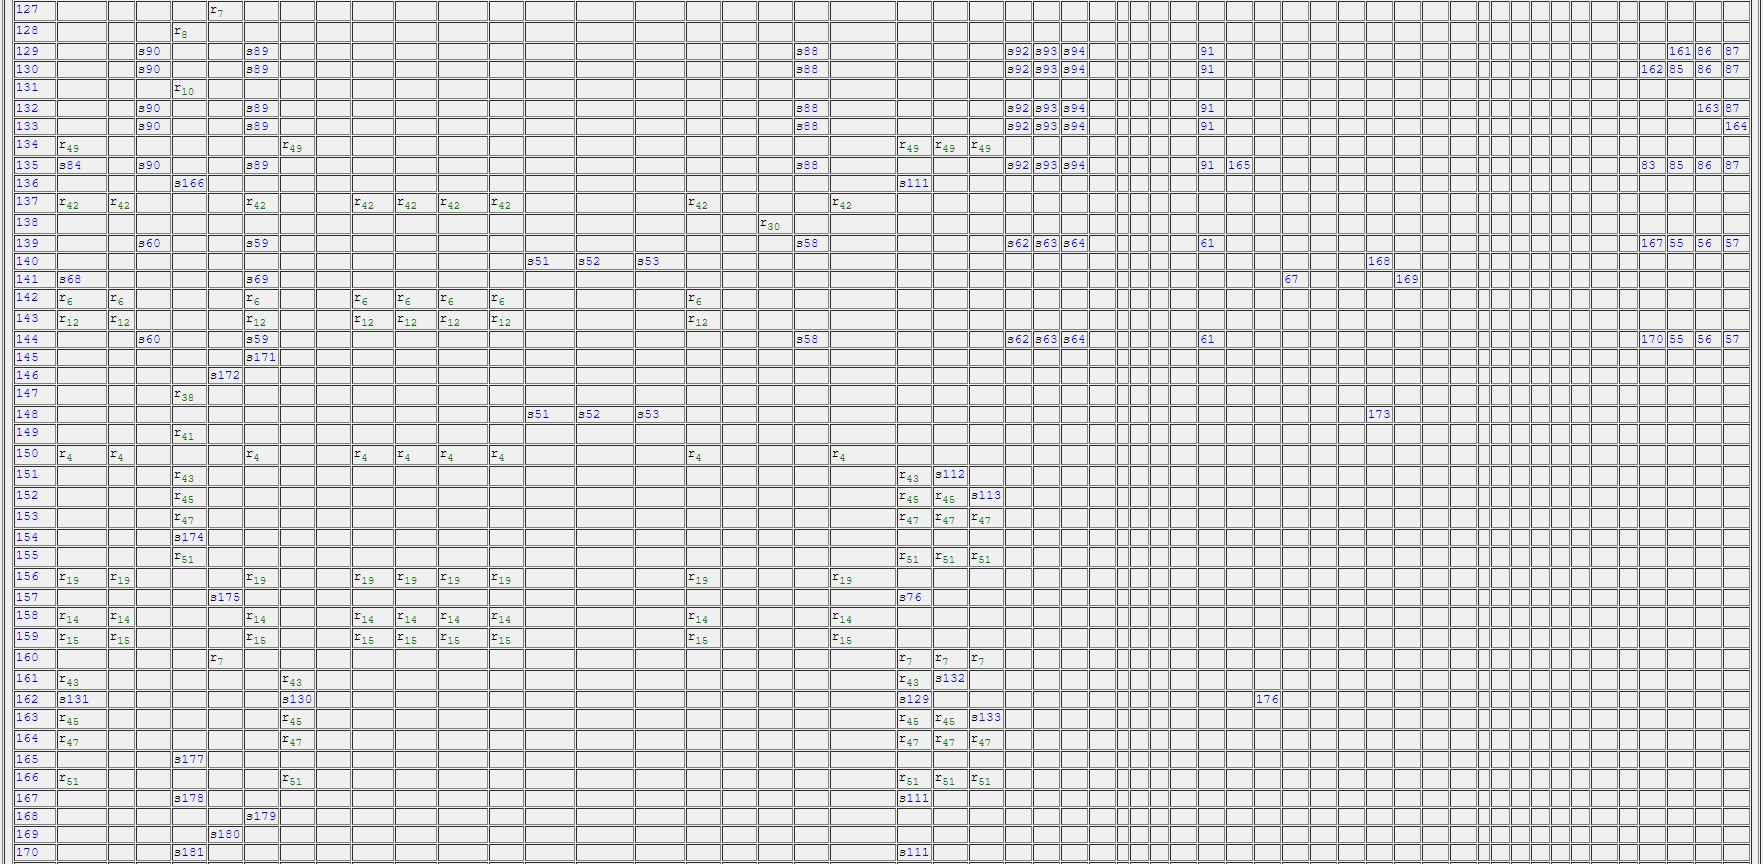
\includegraphics[width=1.27\textwidth]{Tabla4.jpg}
        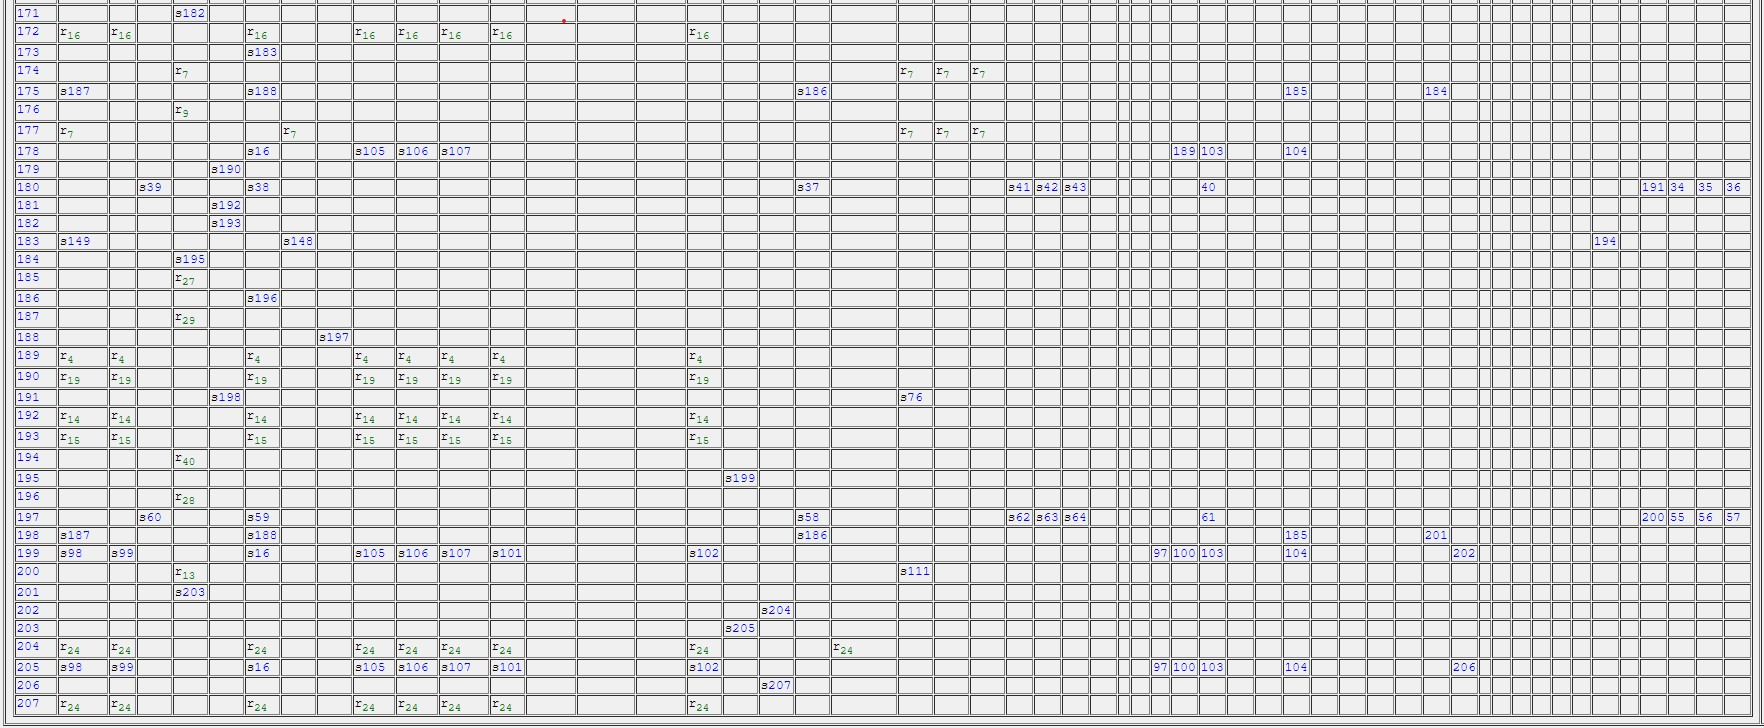
\includegraphics[width=1.27\textwidth]{Tabla5.jpg}
    \end{center}
\end{changemargin}

\vspace{3mm}
Como puede observarse en la tabla\cite{TABLA-LR}, esta gramática es adecuada para este tipo de analizador sintáctico, puesto que no se produce ningún tipo de conflicto.
\clearpage

\section{Diseño Analizador Semántico}
\VerbatimInput{Pseudo-PDL.txt}

\clearpage
\section{Diseño Tabla de Símbolos}

\clearpage
\printbibliography[heading=bibnumbered]



\end{document}